\section{Demo}
\label{sec:demo}

The demo (\texttt{scripts/demo.py}, built with Gradio) is a web application in which a user pastes one clause or a whole Terms of Service and sees what the system decided and why. It runs the evaluated system through the same functions as the experiments, so what the user sees is what we measured. It works with gpt-4.1-mini, with any open-weight model behind an OpenAI-compatible server, or without any language model (\emph{evidence only}, the kNN vote).

\begin{itemize}
  \item \textbf{Check a clause} shows:
    \begin{itemize}
      \item the verdict, the model's explanation, and why this kind of clause matters for consumers;
      \item the cited rationales and provisions, linked to the official texts;
      \item the expert-labelled precedents, with a bar per category that shows how many of the 8 most similar clauses have it and where the threshold of the gate lies;
      \item each step of the decision, the time and the estimated cost.
    \end{itemize}
  \item \textbf{Check a document} splits the text into sentences, with rules for abbreviations in the four languages, and checks each sentence. It lists:
    \begin{itemize}
      \item the flagged clauses, each expandable to the same details;
      \item the \emph{borderline} clauses, which the model flagged but the precedents did not confirm;
    \end{itemize}
    and it highlights the full text (Figures~\ref{fig:demo-flags} and~\ref{fig:demo-text}). The results can be downloaded as a table.
  \item \textbf{About} states that this is an AI system and not legal advice. It shows the measured accuracy of the running model, overall and per language, read from the saved results, together with the limits of the system and where the submitted text goes.
\end{itemize}

\begin{figure}[ht]
\centering
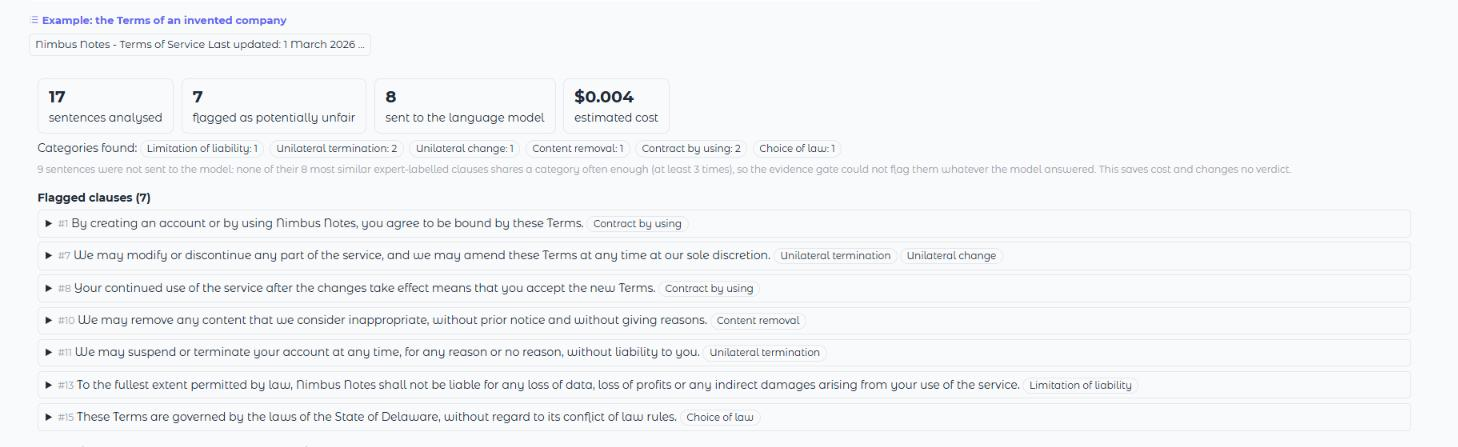
\includegraphics[width=\textwidth]{demo_document_flags.pdf}
\caption{Demo, document mode, with gpt-4.1-mini on the Terms of an invented company written for the demo: summary and flagged clauses.}
\label{fig:demo-flags}
\end{figure}

\begin{figure}[ht]
\centering
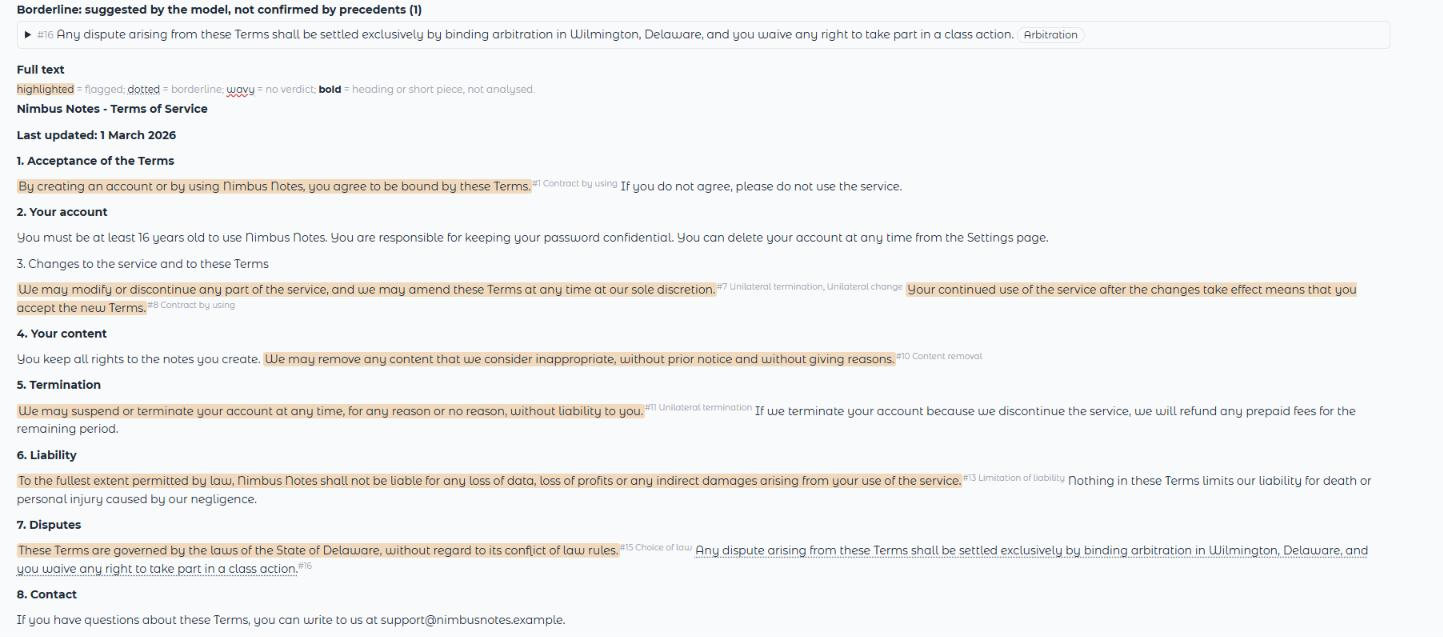
\includegraphics[width=\textwidth]{demo_document_text.pdf}
\caption{Demo, document mode: the borderline arbitration clause, overruled by the gate, and the highlighted full text. The limitation of liability (\#13) is flagged; the next sentence, which preserves liability for personal injury, is correctly left alone.}
\label{fig:demo-text}
\end{figure}

Four design choices follow from our results.
\begin{itemize}
  \item \textbf{The precedents are shown next to the citations.} They separate right from wrong flags better than the citations do (Section~\ref{sec:explanations}).
  \item \textbf{Nothing is hidden or presented as ``fair''.} A flag overruled by the gate appears as borderline, and ``not flagged'' is never worded as ``fair''. A failed model call gives ``no verdict'' and never a silent ``not flagged''.
  \item \textbf{A document costs about a seventh as much, with identical verdicts.} When no category has 3 of the 8 precedents, the gate would remove whatever the model said, so the model is not asked. On the test set only 223 of the 1,607 sentences need the model (13.9\%), and between 12.3\% and 14.3\% in the four languages of the multilingual set; none of the skipped sentences was flagged by the evaluated system. In the run of Figure~\ref{fig:demo-flags}, 8 of 17 sentences were sent to the model, for \$0.004. A single clause is always sent, so that the model's reasoning is visible even when the gate overrules it.
  \item \textbf{Safety and privacy.} All text from the user, the model or the knowledge base is escaped before display, and the demo stores nothing.
\end{itemize}

The example in Figures~\ref{fig:demo-flags} and~\ref{fig:demo-text} was written to contain eight clearly unfair and nine fair sentences. The system flagged seven of the eight, with the intended categories, and raised no false alarm. The eighth, an arbitration clause, was recognised by the model but overruled by the gate, because few of its nearest precedents were arbitration clauses. It is the trade-off of Section~\ref{sec:gate} in a single case, and the reason the demo shows borderline clauses. This is an illustration, not an evaluation: the sentences are ours and so are the intended labels.

The demo has 14 unit tests with a fake embedding model and a fake language model, and it was checked end to end in a headless browser.
